\documentclass[journal,trans]{IEEEtran}
\usepackage[spanish]{babel}
\usepackage[utf8]{inputenc}
\usepackage{graphicx}
\usepackage{amsmath}
\usepackage{amssymb}
\usepackage{multirow}
\usepackage[dvipsnames]{xcolor}
\usepackage{ifpdf}
\usepackage{cite}
\usepackage{url}
\hyphenation{op-tical net-works semi-conduc-tor}

\begin{document}

	\newcommand{\titlepaper}{Proyecto Final}
	
	\title{\titlepaper}
	
	\renewcommand\IEEEkeywordsname{Palabras clave}
	
	\author{\IEEEauthorblockN{Fiorella Delgado León, Jonathan Guzmán Araya, Mariano Muñoz Masís}
	\IEEEauthorblockA{\\fiorelladelgado53@gmail.com, jonathana1196@gmail.com, marianomm1301@gmail.com}
	\IEEEauthorblockA{\\Área Académica de Ingeniería en Computadores}
	\IEEEauthorblockA{\\Instituto Tecnológico de Costa Rica, Cartago, Costa Rica, 2021}
	}
	
	\markboth{Taller de Diseño Digital, \titlepaper}%
	{Shell \MakeLowercase{\textit{et al.}}: Bare Demo of IEEEtran.cls for Journals}
	
	% Note that keywords are not normally used for peerreview papers.
	
	\IEEEtitleabstractindextext{%
	\begin{abstract}
			Este documento presenta los resultados del proyecto final del curso.
	\end{abstract}
	\begin{IEEEkeywords}
		FPGA
	\end{IEEEkeywords}}
	
	% make the title area
	\maketitle
	
	\IEEEdisplaynontitleabstractindextext
	
	\IEEEpeerreviewmaketitle
	
	\section{Introducción}
	
	El procesador ARM es un componente clave de muchos sistemas integrados. El primer ARM se introdujo en 1985, bajo el nombre de Acorn RISC Machine (luego renombrado Advanced RISC Machine). La relativa simplicidad de los procesadores ARM los hizo adecuados para aplicaciones de bajo consumo permitiendo así su actual amplia adopción. ARM es inusual en el sentido de que no vende proesadores directamente, si no que autoriza a otras compañías a construir sus diseños de procesadores, a menudo como parte de un sistema en chip más grande, por ejemplo: Samsung, Altera, Apple, Qualcomm construyen procesadores ARM, ya sea utilizando microarquitecturas compradas en ARM o microarquitecturas desarrolladas bajo licencia ARM \cite{Gomar2018}.
	
	La arquitectura de un computador es la visión del programador de una computadora, esta arquitectura está definida por un conjunto de instrucciones (lenguaje) y ubicaciones de los operandos (registros y memoria) \cite{SarahLHarris2010}. 
	
	El primer paso para entender la arquitectura de un computadora es entender su lenguaje, las palabras en el lenguaje de una computadora son llamadas instrucciones, el vocabulario de una computadora es llamado conjunto de instrucciones, de manera que todos los programas en esta computadora utilizan el mismo conjunto de instrucciones, incluso las más complejas.
	
	\subsection{Tipos de instrucciones y su codificación}
	Las instrucciones de una computadora indican el tipo de operación a realizar y los operandos a utilizar, los operandos vienen desde la memoria a los registros y de estos a las instrucciones. Las computadoras solo comprender 1's y 0's, es por esto que las instrucciones son codificadas en como números binarios en un formato llamado lenguaje máquina \cite{SarahLHarris2010}.
	
	El lenguaje Ensamblador es la representación humana de este lenguaje máquina, cada instrucción en Ensamblador especifica tanto el tipo de instrucción como sus operandos. En ARMv4 existen cuatro formatos principales de instrucciones: data procesing, memory, branch y miscellaneous. Este pequeño número de formatos permite cierta regularidad entre las instrucciones, y por lo tanto, un hardware de decodificador simple \cite{SarahLHarris2010}.
	
	\subsubsection{Data Procesing Instructions}
	Las instrucciones de procesamiento de datos tienen dos registros fuentes, donde el segundo puede ser un inmediato y el tercer registro que es el destino. 
	
	\begin{figure}[h]
		\centering
		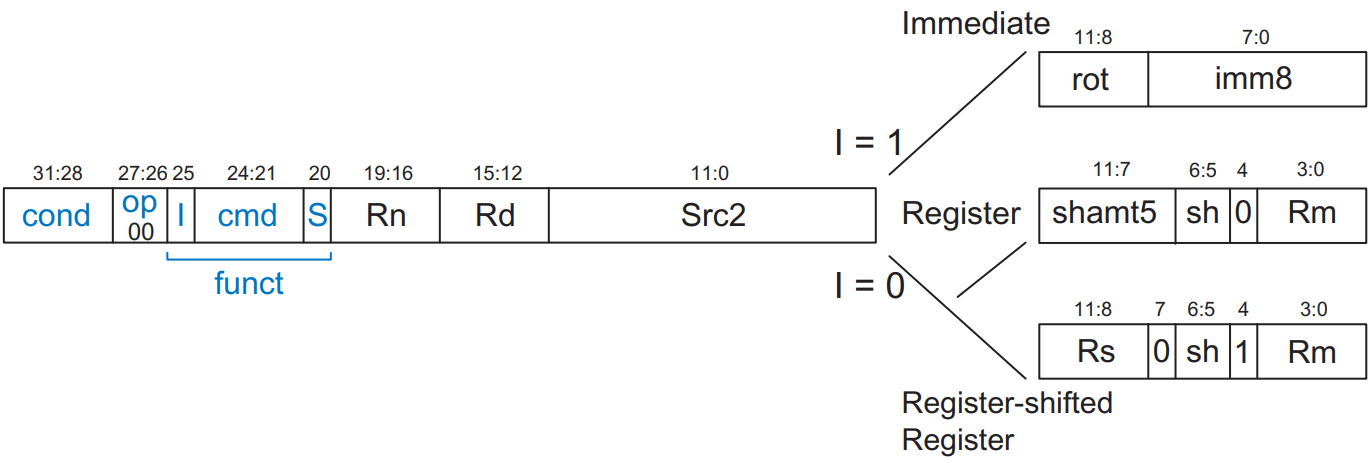
\includegraphics[width=\linewidth]{img/datapro.png}
		\caption{Codificación de instrucciones de procesamiento de datos \cite{SarahLHarris2010}}
		\label{fig:DataP}
	\end{figure}

	Los 32 bits de estos tipos de instrucciones tienen bits específicos asignados para una serie de datos que tienen que ir en esos bits para especificar el tipo de instrucción y que hacer con los mismos, esto se detalla a continuación.
	
	\begin{itemize}
		\item cond: ejecución condicional basada en las banderas que se especificaron en la Tabla \ref{tab:Banderas}.
		\item op: código del tipo operación a realizar.
		\item funct: código de instrucción a realizar, a su vez en las instrucciones de procesamiento de datos este se divide en tres partes.
		\begin{itemize}
			\item I: especifica si se está o no trabajando con un inmediato.
			\item cmd: código de la instrucción a realizar.
			\item S: si las banderas se tienen que guardar o no.
		\end{itemize}
		\item Rn: registro para el operando $1$.
		\item Rd: registro destino donde se guardará el resultado de los operandos.
		\item Src2: en las instrucciones de procesamiento puede presentar tres casos.
		\begin{itemize}
			\item Inmediato
			\begin{itemize}
				\item rot: rotación circular de 8 bits para armar números de 32 bits.
				\item imm8: inmediato, este no puede ser más de 255.
			\end{itemize}
			\item Registro
			\begin{itemize}
				\item shamt5: constante de desplazamiento.
				\item sh: indica el tipo de desplazamiento a realizar como se observa en la Tabla \ref{tab:sh}.
				\item 0: bit por defecto según la instrucción.
				\item Rm: registro para el operando $2$.
			\end{itemize}
			\item Registro con desplazamiento
			\begin{itemize}
				\item Rs: registro de desplazamiento.
				\item 0: bit por defecto según la instrucción.
				\item sh: indica el tipo de desplazamiento a realizar como se observa en la Tabla \ref{tab:sh}.
				\item 1: bit por defecto según el tipo de instrucción.
				\item Rm: registro para el operando $2$.
			\end{itemize}
		\end{itemize}
	\end{itemize}

	\begin{table}[h]
		\centering
		\begin{tabular}{|c|c|c|}
			\hline
			Instrucción & sh       & Operación \\
			\hline
			\hline
			LSL         & $00_{2}$ & Logical left shift \\
			\hline
			LSR         & $01_{2}$ & Logical right shift \\
			\hline
			ASR         & $10_{2}$ & Arithmetic shift right \\
			\hline
			ROR         & $11_{2}$ & Rotate right \\
			\hline
		\end{tabular}
		\caption{Código de operación de sh}
		\label{tab:sh}
	\end{table}
	
	\subsubsection{Memory Instructions}
	Las instrucciones de memoria utilizan un formato similar al que utilizan las instrucciones de procesamiento de datos, con las mimas seis divisiones, sin embargo, utilizan un código de operación diferente al utilizado en las instrucciones de procesamiento de datos tal y como se muestra en la Figura \ref{fig:MemoryP}.
	
	\begin{figure}[h]
		\centering
		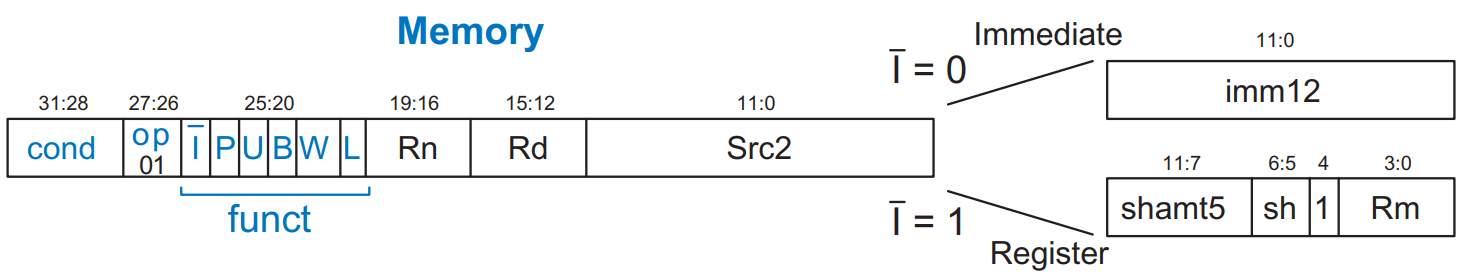
\includegraphics[width=\linewidth]{img/mempro.png}
		\caption{Codificación de instrucciones de memoria \cite{SarahLHarris2010}}
		\label{fig:MemoryP}
	\end{figure}
	
	\begin{itemize}
		\item cond: ejecución condicional basada en las banderas que se especificaron en la Tabla \ref{tab:Banderas}.
		\item op: código del tipo operación a realizar.
		\item funct: código de instrucción a realizar, a su vez está compuesto de seis bits de control.
		\begin{itemize}
			\item $\overline{I}$ - U: Los bits $\overline{I}$ (inmediato) y U (sumar) determinan si el desplazamiento es inmediato o de registro y si se debe sumar o restar de acuerdo a la Tabla \ref{tab:IU}.
			\item P - W: Los bits P (pre-índice) y W (escritura) especifican el modo de índice de acuerdo a la Tabla \ref{tab:PW}.
			\item B - L: Los bits L (carga) y B (byte) especifican el tipo de operación de memoria de acuerdo a la Tabla \ref{tab:LB}.
		\end{itemize}
		\item Rn: registro para el operando $1$.
		\item Rd: registro destino donde se guardará el resultado de los operandos.
		\item Src2: en las instrucciones de memoria puede presentar dos casos.
		\begin{itemize}
			\item Inmediato
			\begin{itemize}
				\item imm12: desplazamiento inmediato sin signo.
			\end{itemize}
			\item Registro
			\begin{itemize}
				\item shamt5: constante de desplazamiento.
				\item sh: indica el tipo de desplazamiento a realizar como se observa en la Tabla \ref{tab:sh}.
				\item 1: bit por defecto según la instrucción.
				\item Rm: registro para el operando $2$.
			\end{itemize}
		\end{itemize}
	\end{itemize}
	
	\begin{table}[h]
		\centering
		\begin{tabular}{|c|c|c|}
			\hline
			Bit & $\overline{I}$           & U \\
			\hline
			\hline
			0   & Desplazamiento inmediato & Restar \\
			\hline
			1   & Registro                 & Sumar \\
			\hline
		\end{tabular}
		\caption{Instrucciones de control para $\overline{I}$ y U}
		\label{tab:IU}
	\end{table}
	
	\begin{table}[h]
		\centering
		\begin{tabular}{|c|c|c|}
			\hline
			P & W & Modo \\
			\hline
			\hline
			0 & 0 & Pos-índice \\
			\hline
			0 & 1 & No soportado \\
			\hline
			1 & 0 & Offset \\
			\hline
			1 & 1 & Pre-índice \\
			\hline
		\end{tabular}
		\caption{Instrucciones de control para P y W}
		\label{tab:PW}
	\end{table}
	
	\begin{table}[!htb]
		\centering
		\begin{tabular}{|c|c|c|}
			\hline
			L & B & Instrucción \\
			\hline
			\hline
			0 & 0 & STR \\
			\hline
			0 & 1 & STRB \\
			\hline
			1 & 0 & LDR \\
			\hline
			1 & 1 & LDRB \\
			\hline
		\end{tabular}
		\caption{Instrucciones de control para L y B}
		\label{tab:LB}
	\end{table}

	\subsubsection{Branch Instructions}
	Las instrucciones de bifurcación utilizan un desplazamiento de 24 bits, por lo que los 32 bits quedan divididos como se muestra en la Figura \ref{fig:BranchP}.
	
	\begin{itemize}
		\item cond: ejecución condicional basada en las banderas que se especificaron en la Tabla \ref{tab:Banderas}.
		\item op: código del tipo operación a realizar.
		\item funct: código de instrucción a realizar.
		\begin{itemize}
			\item 1L: su tamaño siempre es de 2 bits y el MSB siempre es 1, mientras que el LSB indica el tipo de bifurcación a realizar.
		\end{itemize}
		\item imm24: se utiliza para especificar la dirección de una dirección de instrucción relativa a $PC + 8$.
	\end{itemize}
	
	\begin{figure}[h]
		\centering
		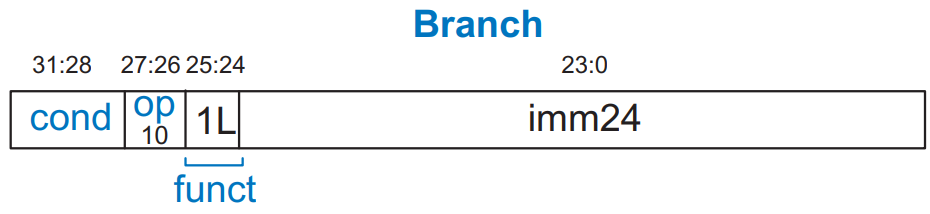
\includegraphics[width=\linewidth]{img/brpro.png}
		\caption{Codificación instrucciones de bifurcación \cite{SarahLHarris2010}}
		\label{fig:BranchP}
	\end{figure}

	\subsubsection{Miscellaneous Instructions}
	El conjunto de instrucciones de ARMv4 tiene otro grupo que se detalla en la Tabla \ref{tab:MISCP}.
	
	\begin{table}[h]
		\centering
		\begin{tabular}{|p{2cm}|p{3cm}|p{3cm}|}
			\hline
			Instrucciones            & Descripción                             & Propósito \\
			\hline
			\hline
			LDM, STM                 & cargar/guardar múltiple                 & Guardar y recuperar registros en llamadas de subrutina \\
			\hline
			SWP, SWPB                & Intercambiar byte                       & Carga atómica y almacenamiento para sincronización de procesos \\
			\hline
			LDRT, LDRBT, STRT, STRBT & cargar/guardar palabra/byte con traslado & Permitir que el sistema operativo acceda a la memoria en el espacio de memoria virtual del usuario \\
			\hline
			SWI                      & Interrupción de software                & Crear una excepción, que a menudo se usa para llamar al sistema operativo \\
			\hline
			CDP, LDC, MCR, MRC, STC  & Acceso de coprocesador                  & Comunicarse con coprocesador opcional \\
			\hline
			MRS, MSR                 & Mover desde/a registro de estado        & Guardar el registro de estado durante las excepciones \\
			\hline
		\end{tabular}
		\caption{Instrucciones misceláneas}
		\label{tab:MISCP}
	\end{table}


	Las instrucciones ARM opcionalmente establecen indicadores de condición en función del resultado Las instrucciones posteriores se ejecutan condicionalmente, dependiendo del estado de esos indicadores, también llamados indicadores de estado que se observan en la Tabla \ref{tab:Banderas}.
	
	\begin{table}[h]
		\centering
		\begin{tabular}{|c|c|p{4.5cm}|}
			\hline
			Bandera & Nombre         & Descripción \\
			\hline
			\hline
			N       & Negativo       & La instrucción resulta negativa si el bit 31 del resultado es $1$ \\
			\hline
			Z       & Cero           & El resultado es 0 \\
			\hline
			C       & Acarreo        & La instrucción provoca acarreo \\
			\hline
			V       & Desbordamiento & La instrucción causa desbordamiento \\
			\hline
		\end{tabular}
		\caption{Banderas}
		\label{tab:Banderas}
	\end{table}

	Estas banderas se activan dependiendo del tipo de instrucción que se esté ejecutando, en la Tabla \ref{tab:FlagsInstructions} se detallan las instrucciones y los tipos de banderas que estos activarían. 
	
	\begin{table}[h]
		\centering
		\begin{tabular}{|c|p{5cm}|c|}
			\hline
			Tipo      & Instrucciones                              & Banderas   \\
			\hline
			\hline
			Add      & ADDS, ADCS                                 & N, Z, C, V \\
			\hline
			Subtract & SUBS, SBCS, RSBS, RSCS                     & N, Z, C, V \\
			\hline
			Compare  & CMP, CMN                                   & N, Z, C, V \\
			\hline
			Shifts   & ASRS, LSLS, LSRS, RORS, RRXS               & N, Z, C    \\
			\hline
			Logical  & ANDS, ORRS, EORS, BICS                     & N, Z, C    \\
			\hline
			Test     & TEQ, TST                                   & N, Z, C    \\
			\hline
			Move     & MOVS, MVNS                                 & N, Z, C    \\
			\hline
			Multiply & MULS, MLAS, SMLALS, SMULLS, UMLALS, UMULLS & N, Z       \\
			\hline
		\end{tabular}
		\caption{Instrucciones que activan las banderas}
		\label{tab:FlagsInstructions}
	\end{table}
	
	La ALU establece estos indicadores y se mantienen en los cuatro bits superiores del CPSR de32 bits tal y como se muestra en la Figura, mientras que los cinco bits menos significativos son los bits de modo, esto es porque un procesador ARM puede operar en una serie de modos de ejecución con diferentes niveles de privilegios. Los diferentes modos permiten que excepciones tomen lugar sin dañar el estado en que se encuentra. Estos modos están especificados en la parte baja del CPSR como se muestra en la Figura \ref{fig:Banderas}y se detallan en Tabla \ref{tab:Modos}.
	
	\begin{figure}[h]
		\centering
		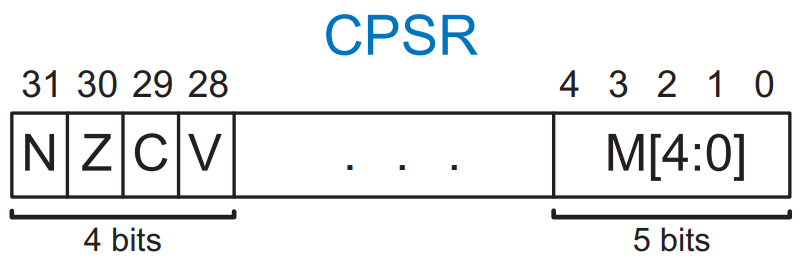
\includegraphics[width =\linewidth]{img/CPSR.png}
		\caption{Bits de las banderas \cite{SarahLHarris2010}}
		\label{fig:Banderas}
	\end{figure}
	
	\begin{table}[h]
		\centering
		\begin{tabular}{|c|c|}
			\hline
			Modo           &  $CPSR_{4:0}$ \\
			\hline
			\hline
			User           &  10000 \\
			\hline
			Supervisor     &  10011 \\
			\hline
			Abort          &  10111 \\
			\hline
			Undefined      &  11011 \\
			\hline
			Interrupt      &  10010 \\
			\hline
			Fast interrupt &  10001 \\
			\hline
		\end{tabular}
		\caption{Modos del procesador}
		\label{tab:Modos}
	\end{table}
		
	\subsection{Registros}
	Las instrucciones 
	
	\subsection{Memoria}
	En la memoria
	
	\section{Sistema Desarrollado}
	Para el desarrollo de este proyecto, se realizó la implementación de una micro arquitectura, utilizando un procesador ARMv4, para descifrar el texto introducido (el cual estará cifrado) mediante uno de los tres algoritmos de descifrado, por medio del lenguaje System Verilog.
	
	\section{Resultados}
	
	\section{Análisis de Resultados}
	
	\section{Conclusiones}
	Al desarrollar este proyecto, se obtuvieron las siguientes conclusiones:
	
	\section{Bibliografía}
	
	\bibliographystyle{IEEEtran}
	\bibliography{myref}
	
\end{document}